\documentclass{beamer}
\usepackage[utf8]{inputenc}
\usepackage{graphicx, epsfig}
\usepackage{amsmath,mathrsfs,amsfonts,amssymb}
%\usepackage{subfig}
\usepackage{floatflt}
\usepackage{epic,ecltree}
\usepackage{mathtext}
\usepackage{fancybox}
\usepackage{fancyhdr}
\usepackage{multirow}
\usepackage{enumerate}
\usepackage{epstopdf}
\usepackage{multicol}
\usepackage{algorithm}
\usepackage[noend]{algorithmic}
\def\algorithmicrequire{\textbf{Input:}}
\def\algorithmicensure{\textbf{Output:}}
\usetheme{default}%{Singapore}%{Warsaw}%{Warsaw}%{Darmstadt}
\usecolortheme{default}
\setbeamertemplate{footline}[page number]{}
\setbeamerfont{title}{size=\Huge}

\newcommand{\bt}{\mathbf{t}} 
\newcommand{\bu}{\mathbf{u}} 
\newcommand{\bv}{\mathbf{v}} 
\newcommand{\bw}{\mathbf{w}} 
\newcommand{\bx}{\mathbf{x}} 
\newcommand{\bz}{\mathbf{z}} 
\newcommand{\by}{\mathbf{y}} 

\newcommand{\bI}{\mathbf{I}} 
\newcommand{\bT}{\mathbf{T}} 
\newcommand{\bX}{\mathbf{X}} 
\newcommand{\bZ}{\mathbf{Z}} 

\newcommand{\bepsilon}{\boldsymbol{\epsilon}}
\newcommand{\bmu}{\boldsymbol{\mu}}
\newcommand{\blambda}{\boldsymbol{\lambda}}
\newcommand{\bsigma}{\boldsymbol{\sigma}}
\newcommand{\bSigma}{\boldsymbol{\Sigma}}

\newcommand{\bbE}{\mathbb{E}} 
\newcommand{\bbP}{\mathbb{P}} 
\newcommand{\bbR}{\mathbb{R}} 

\newcommand{\cL}{\mathcal{L}} 
\newcommand{\cN}{\mathcal{N}} 
\newcommand{\cS}{\mathcal{S}} 
\newcommand{\cX}{\mathcal{X}} 

\newcommand{\btheta}{\boldsymbol{\theta}} 
\newcommand{\bphi}{\boldsymbol{\phi}} 

\DeclareMathOperator*{\argmin}{arg\,min}
\DeclareMathOperator*{\argmax}{arg\,max}

%\definecolor{beamer@blendedblue}{RGB}{15,120,80}
%----------------------------------------------------------------------------------------------------------
\title[\hbox to 56mm{Deep Generative Models  \hfill\insertframenumber\,/\,\inserttotalframenumber}]
{Deep Generative Models \\ Lecture 8}
\author[Roman Isachenko]{\\Roman Isachenko}
\institute[MIPT]{Moscow Institute of Physics and Technology \\
}
\date{2020}
%--------------------------------------------------------------------------------
\begin{document}
%--------------------------------------------------------------------------------
\begin{frame}
%\thispagestyle{empty}
\titlepage
\end{frame}
%=======
\begin{frame}{Generative models zoo}
\begin{figure}
	\centering
	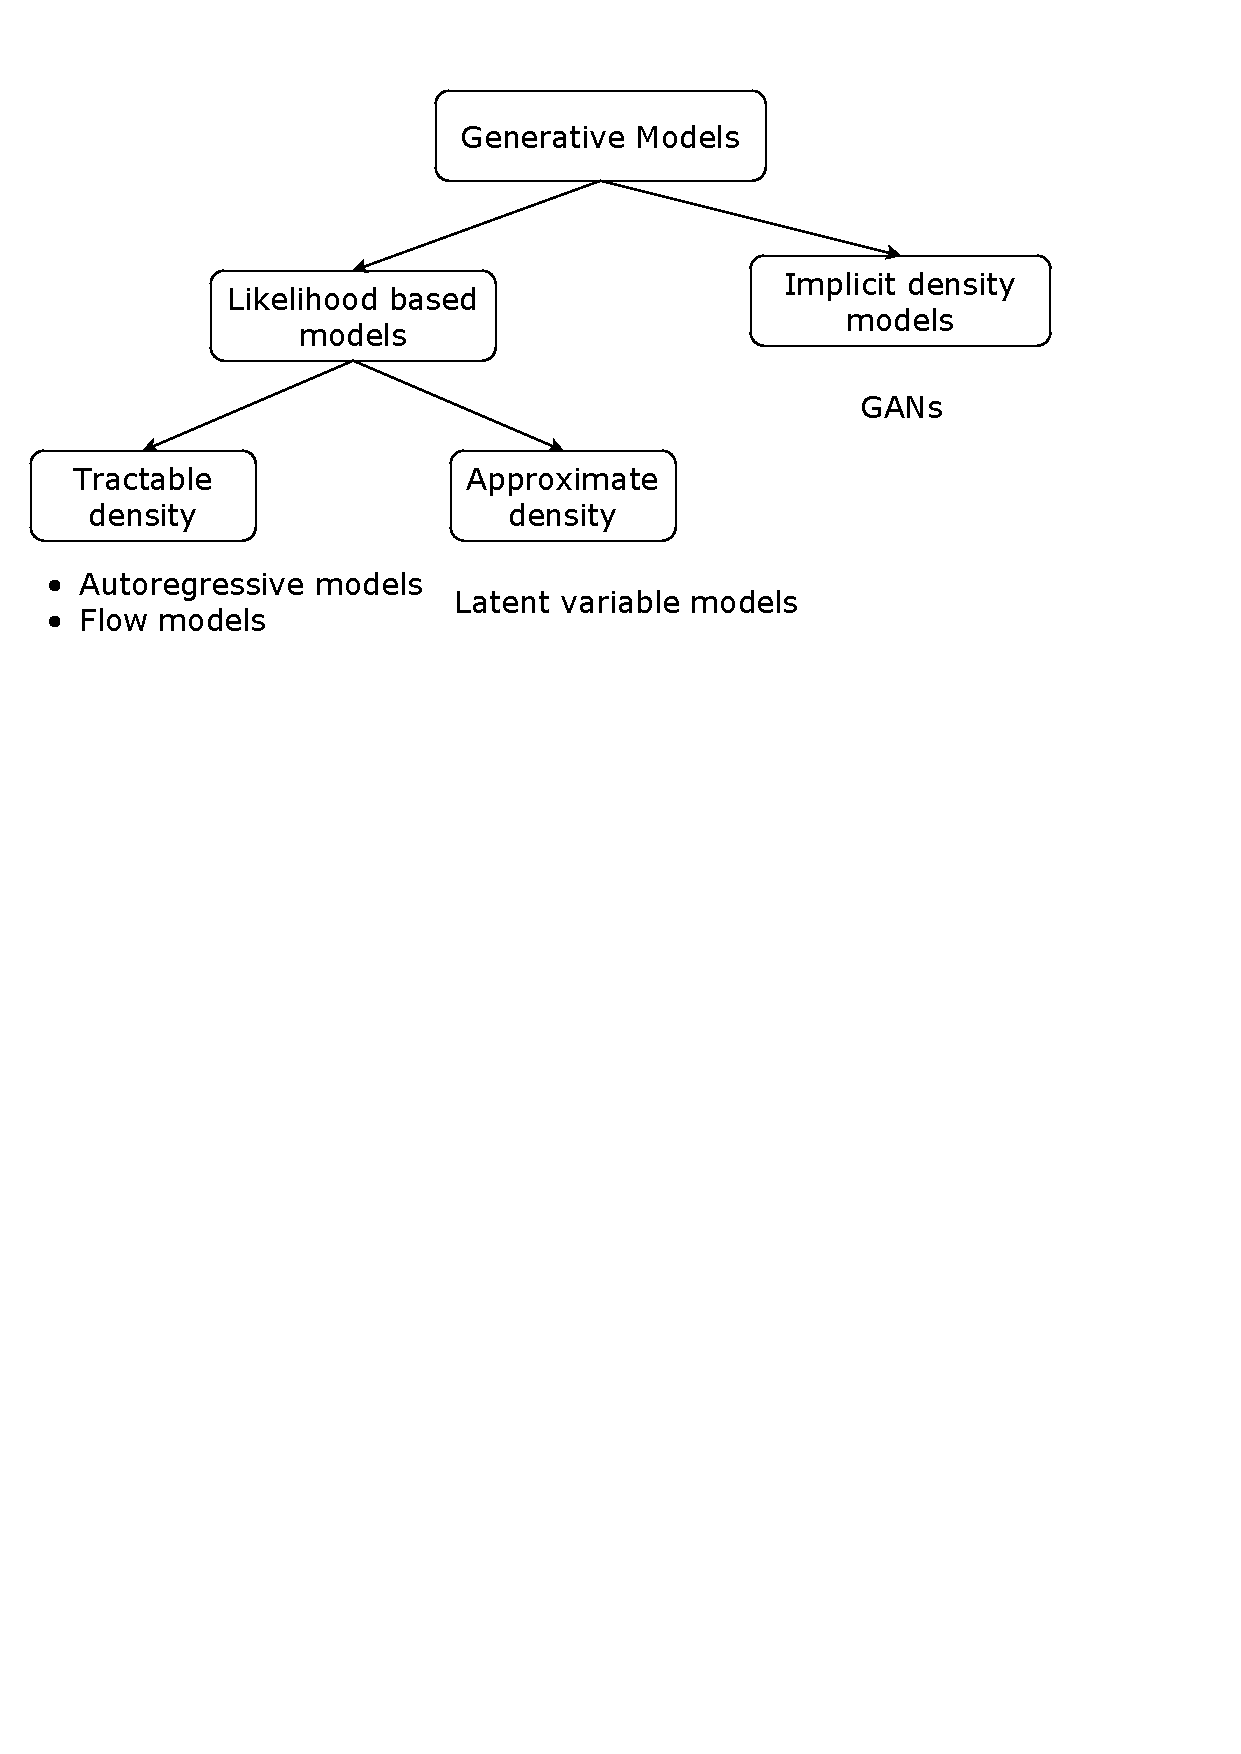
\includegraphics[width=1.0\linewidth]{figs/generative_models_zoo.pdf}
\end{figure}
\end{frame}
%=======
\begin{frame}{Likelihood based models}
	Is likelihood a good measure of model quality?
	\begin{minipage}[t]{0.48\columnwidth}
		\begin{block}{Poor likelihood \\ Great samples}
			\vspace{-0.3cm}
			\[
				p_1(\bx) = \frac{1}{n} \sum_{i=1}^n \cN(\bx | \bx_i, \epsilon \bI)
			\]
			For small $\epsilon$ this model will generate samples with great quality, but likelihood will be very poor.
		\end{block}
	\end{minipage}%
	\begin{minipage}[t]{0.52\columnwidth}
		\begin{block}{Great likelihood \\ Poor samples}
			\vspace{-0.3cm}
			\[
				p_2(\bx) = 0.01p(\bx) + 0.99p_{\text{noise}}(\bx)
			\]
			\begin{multline*}
				\log \left[ 0.01p(\bx) + 0.99p_{\text{noise}}(\bx) \right] \geq  \\ \geq \log \left[ 0.01p(\bx) \right]  = \log p(\bx) - \log 100
			\end{multline*}
		Noisy irrelevant samples, but for high dimensions $\log p(\bx)$ becames larger.
		\end{block}
	\end{minipage}
	\vfill
	\hrule\medskip
	{\scriptsize \href{https://arxiv.org/abs/1511.01844}{https://arxiv.org/abs/1511.01844}}
\end{frame}
%=======
\begin{frame}{Likelihood-free learning}
	\begin{itemize}
		\item Likelihood is not a perfect measure for quality measure for generative model.
		\item Likelihood could be intractable.
	\end{itemize}
	\begin{block}{Where did we start}
	 We would like to approximate true data distribution $\pi(\bx)$.
		Instead of searching true $\pi(\bx)$ over all probability distributions, learn function approximation $p(\bx | \btheta) \approx \pi(\bx)$.
	\end{block}
	Imagine we have two sets of samples 
	\begin{itemize}
		\item $\cS_1 = \{\bx_i\}_{i=1}^{n_1} \sim \pi(\bx)$
		\item $\cS_2 = \{\bx_i\}_{i=1}^{n_2} \sim p(\bx | \btheta)$
	\end{itemize}
	\begin{block}{Two sample test}
		\vspace{-0.3cm}
		\[
			H_0: \pi(\bx) = p(\bx | \btheta), \quad H_1: \pi(\bx) \neq p(\bx | \btheta)
		\]
	\end{block}

\end{frame}
%=======
\begin{frame}{Likelihood-free learning}
		\begin{block}{Two sample test}
			\vspace{-0.3cm}
			\[
				H_0: \pi(\bx) = p(\bx | \btheta), \quad H_1: \pi(\bx) \neq p(\bx | \btheta)
			\]
	\end{block}
	Define test statistic $T(\cS_1, \cS_2)$. Test statictic is likelihood free.
	
	If $T(\cS_1, \cS_2) < \alpha$, then accept $H_0$, else reject it.
	
	\begin{block}{Desired behaviour}
		\begin{itemize}
			\item The generative model $p(\bx | \btheta)$ minimizes the value of test statistic~$T(\cS_1, \cS_2)$.
			\item Find appropriate test statistic in high dimensions is hard. We could try to learn the appropriate $T(\cS_1, \cS_2)$.
		\end{itemize}
	\end{block}
\end{frame}
%=======
\begin{frame}{Vanila GAN}
	\begin{itemize}
		\item \textbf{Generator:} latent variable model $\bx = G(\bz)$, which minimizes two-sample test objective.
		\item \textbf{Discriminator:} function $D(\bx)$, which distinguish real samples from model samples and maximizes two-sample test statistic.
	\end{itemize}
	\begin{block}{Objective}
		\[
			V(G, D) = \min_{G} \max_D \bbE_{\pi(\bx)} \log D(\bx) + \bbE_{p(\bz)} \log (1 - D(G(\bz)))
		\]
	\end{block}
	For fixed generator $G(\bz)$ discriminator is performing binary classification with cross entropy loss.
	
	 This minimax game has global optimum $\pi(\bx) = p(\bx | \btheta)$.
	 \vfill
	 \hrule\medskip
	 {\scriptsize \href{https://arxiv.org/abs/1406.2661}{https://arxiv.org/abs/1406.2661}}
\end{frame}
%=======
\begin{frame}{Vanila GAN optimality}
	
	\begin{block}{Objective (fixed $G$)}
		\[
		\max_D V(D) = \bbE_{\pi(\bx)} \log D(\bx) + \bbE_{p(\bz)} \log (1 - D(G(\bz)))
		\]
	\end{block}
	\begin{block}{Optimal discriminator}
		\vspace{-0.5cm}
		\begin{align*}
			V(G, D) &= \bbE_{\pi(\bx)} \log D(\bx) + \bbE_{p(\bx | \btheta)} \log (1 - D(\bx)) \\
			&= \int \underbrace{\left[ \pi(\bx) \log D(\bx) + p(\bx | \btheta)\log (1 - D(\bx) \right]}_{y(D)} d \bx
		\end{align*}
		\[
			\frac{d y(D)}{d D} = \frac{\pi(\bx)}{D(\bx)} - \frac{p(\bx | \btheta)}{1 - D(\bx)} = 0 \quad \Rightarrow \quad D^*(\bx) = \frac{\pi(\bx)}{\pi(\bx) + p(\bx | \btheta)}
		\]
	\end{block}
	\vfill
	\hrule\medskip
	{\scriptsize \href{https://arxiv.org/abs/1406.2661}{https://arxiv.org/abs/1406.2661}}

\end{frame}
%=======
\begin{frame}{Vanila GAN optimality}
	
	\begin{block}{Objective (fixed $D$)}
		\[
		\max_G V(G, D^*) = \bbE_{\pi(\bx)} \log D^*(\bx) + \bbE_{p(\bz)} \log (1 - D^*(G(\bz)))
		\]
	\end{block}
	\begin{block}{Optimal generator}
		\vspace{-0.5cm}
		\begin{multline*}
			V(G, D^*) = \bbE_{\pi(\bx)} \log \frac{\pi(\bx)}{\pi(\bx) + p(\bx | \btheta)} + \bbE_{p(\bx | \btheta)} \log \frac{p(\bx | \btheta)}{\pi(\bx) + p(\bx | \btheta)} \\
			 = KL \left(\pi(\bx) || \frac{\pi(\bx) + p(\bx | \btheta)}{2}\right) + KL \left(p(\bx | \btheta) || \frac{\pi(\bx) + p(\bx | \btheta)}{2}\right) - 2\log 2 \\
			 = 2JSD(\pi(\bx) || p(\bx | \btheta)) - 2\log 2.
		\end{multline*}
	\end{block}
	\vfill
	\hrule\medskip
	{\scriptsize \href{https://arxiv.org/abs/1406.2661}{https://arxiv.org/abs/1406.2661}}
	
\end{frame}
%=======
\begin{frame}{Vanila GAN optimality}
	\begin{block}{Optimal generator}
		\vspace{-0.2cm}
		\[
			V(G, D^*)  = 2JSD(\pi(\bx) || p(\bx | \btheta)) - 2\log 2.
		\]
	\end{block}
	\begin{block}{Jensen-Shannon divergence}
		\vspace{-0.2cm}
		\footnotesize
		\[
			JSD(\pi(\bx) || p(\bx | \btheta)) = \frac{1}{2} \left[KL \left(\pi(\bx) || \frac{\pi(\bx) + p(\bx | \btheta)}{2}\right) + KL \left(p(\bx | \btheta) || \frac{\pi(\bx) + p(\bx | \btheta)}{2}\right) \right]
		\]
	\end{block}
	Also called symmetric KL divergence. Could be used as a distance measure!
	
	\[
		V(G^*, D^*) = -2\log 2, \quad \pi(\bx) = p(\bx | \btheta).
	\]
	If the generator updates are made in function space and discriminator is optimal at every step, then the generator is
	guaranteed to converge to the data distribution.
\end{frame}
%=======
\begin{frame}{Vanila GAN}
	\begin{block}{Objective}
		\vspace{-0.4cm}
		\[
		V(G, D) = \min_{G} \max_D \bbE_{\pi(\bx)} \log D(\bx) + \bbE_{p(\bz)} \log (1 - D(G(\bz)))
		\]
		\vspace{-0.4cm}
	\end{block}

	\begin{figure}
		\centering
		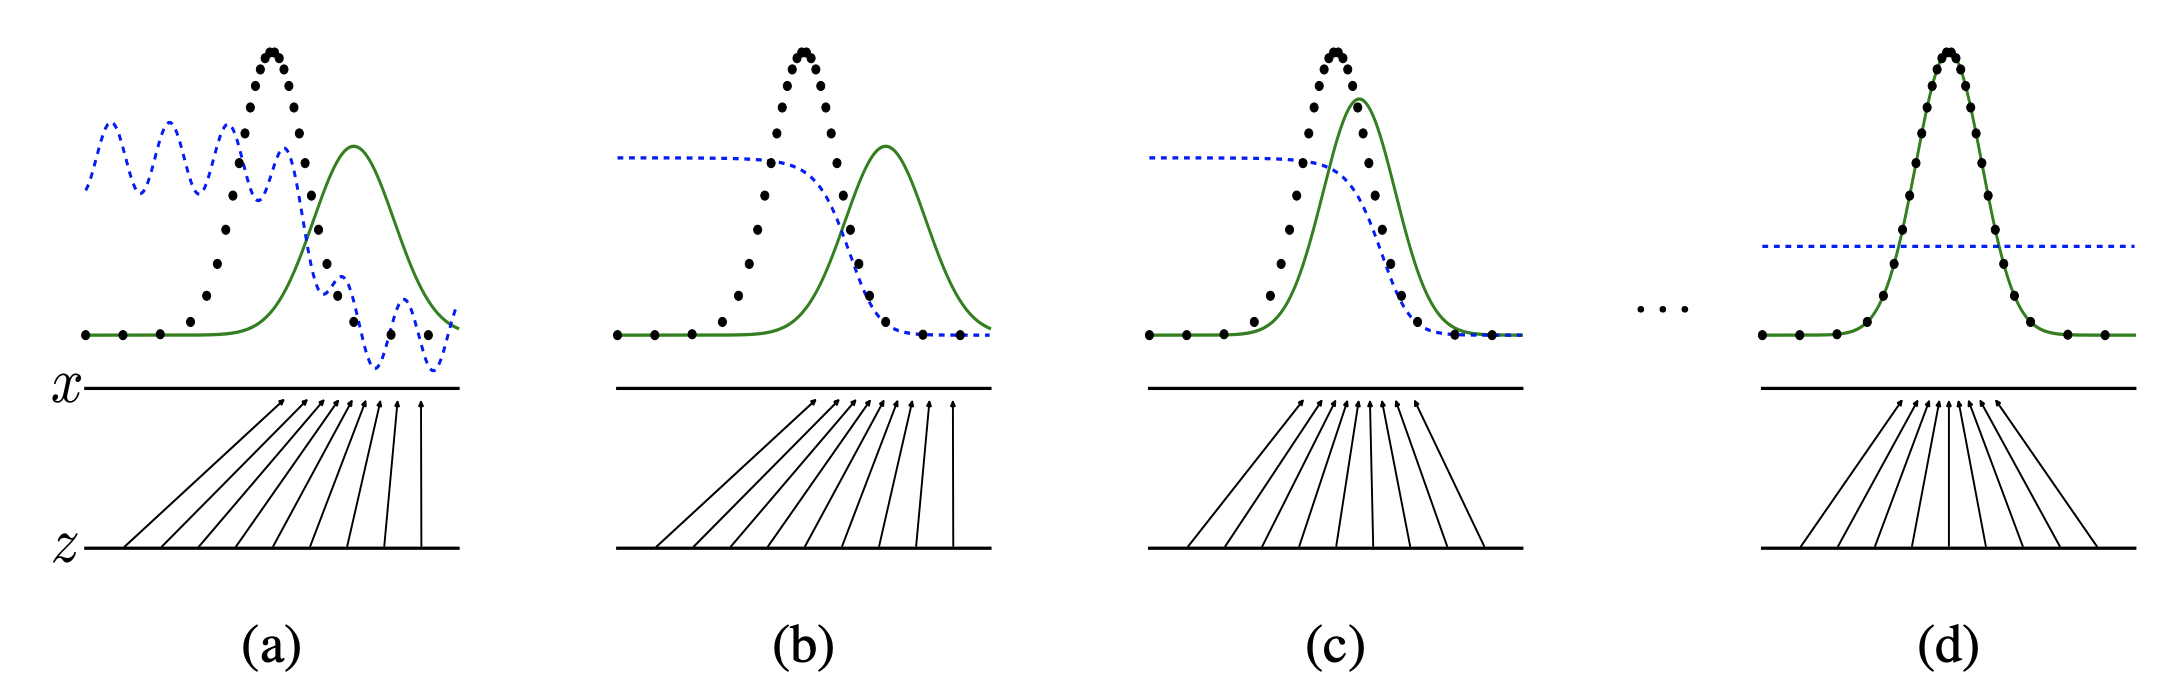
\includegraphics[width=1.0\linewidth]{figs/gan_1}
	\end{figure}
	\begin{itemize}
		\item Generator updates are made in parameter space.
		\item Discriminator is not optimal at every step.
		\item Generator and discriminator loss keeps oscillating during GAN training.
	\end{itemize}
	\vfill
	\hrule\medskip
	{\scriptsize \href{https://arxiv.org/abs/1406.2661}{https://arxiv.org/abs/1406.2661}}
\end{frame}
%=======
\begin{frame}{Vanishing gradients}
	\begin{block}{Objective}
		\vspace{-0.4cm}
		\[
		V(G, D) = \min_{G} \max_D \bbE_{\pi(\bx)} \log D(\bx) + \bbE_{p(\bz)} \log (1 - D(G(\bz)))
		\]
		\vspace{-0.4cm}
	\end{block}
	Early in learning, $G$ is poor, $D$ can reject samples with high confidence. In this case, $\log (1 - D(G(\bz)))$ saturates.
	\begin{minipage}[t]{0.5\columnwidth}
		\begin{figure}
			\centering
			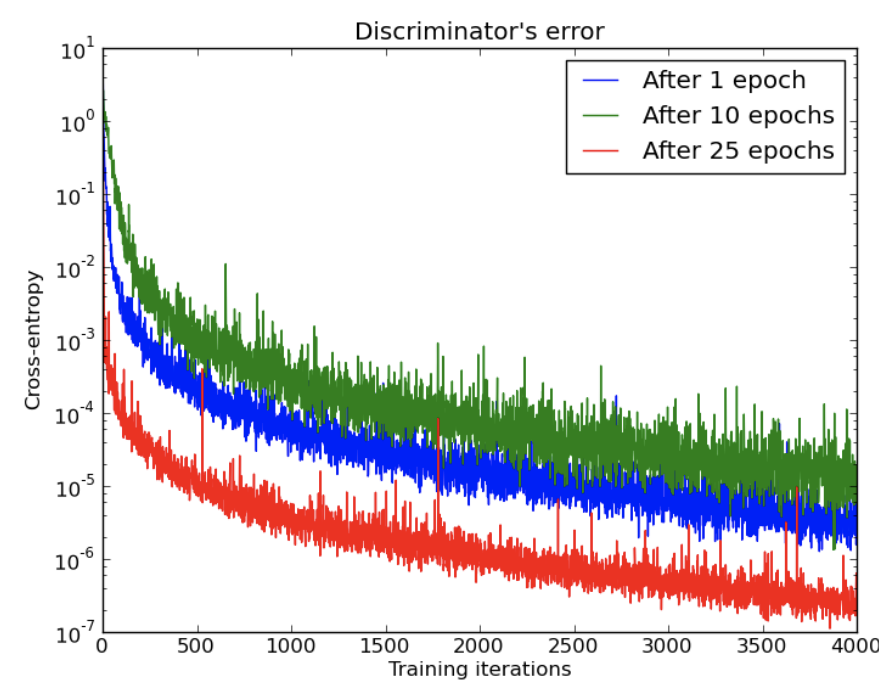
\includegraphics[width=0.9\linewidth]{figs/vanishing_gradients_1}
		\end{figure}
	\end{minipage}%
	\begin{minipage}[t]{0.5\columnwidth}
		\begin{figure}
			\centering
			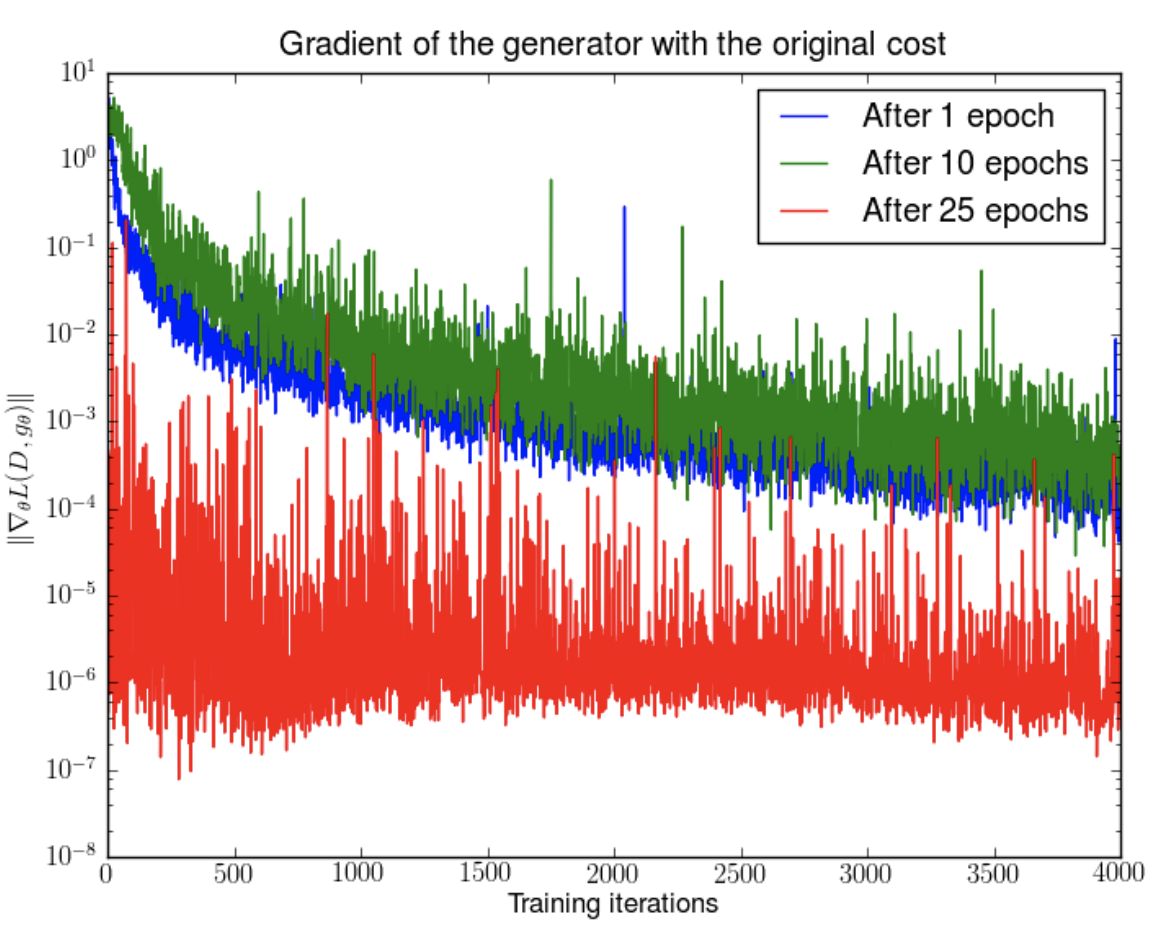
\includegraphics[width=0.9\linewidth]{figs/vanishing_gradients_2}
		\end{figure}
	\end{minipage}
	\vfill
	\hrule\medskip
	{\scriptsize \href{https://arxiv.org/abs/1701.04862}{https://arxiv.org/abs/1701.04862}}
\end{frame}
%=======
\begin{frame}{Vanishing gradients}
	\begin{block}{Objective}
		\vspace{-0.4cm}
		\[
		V(G, D) = \min_{G} \max_D \bbE_{\pi(\bx)} \log D(\bx) + \bbE_{p(\bz)} \log (1 - D(G(\bz)))
		\]
		\vspace{-0.4cm}
	\end{block}
	\begin{minipage}[t]{0.45\columnwidth}
		\vspace{0.4cm}
		Maximize $\log D(G(z))$ instead of $\log (1 - D(G(\bz)))$. \\
		Gradients are getting much stronger, but the training is instable (with increasing mean and variance).
	\end{minipage}%
	\begin{minipage}[t]{0.55\columnwidth}
		\begin{figure}
			\centering
			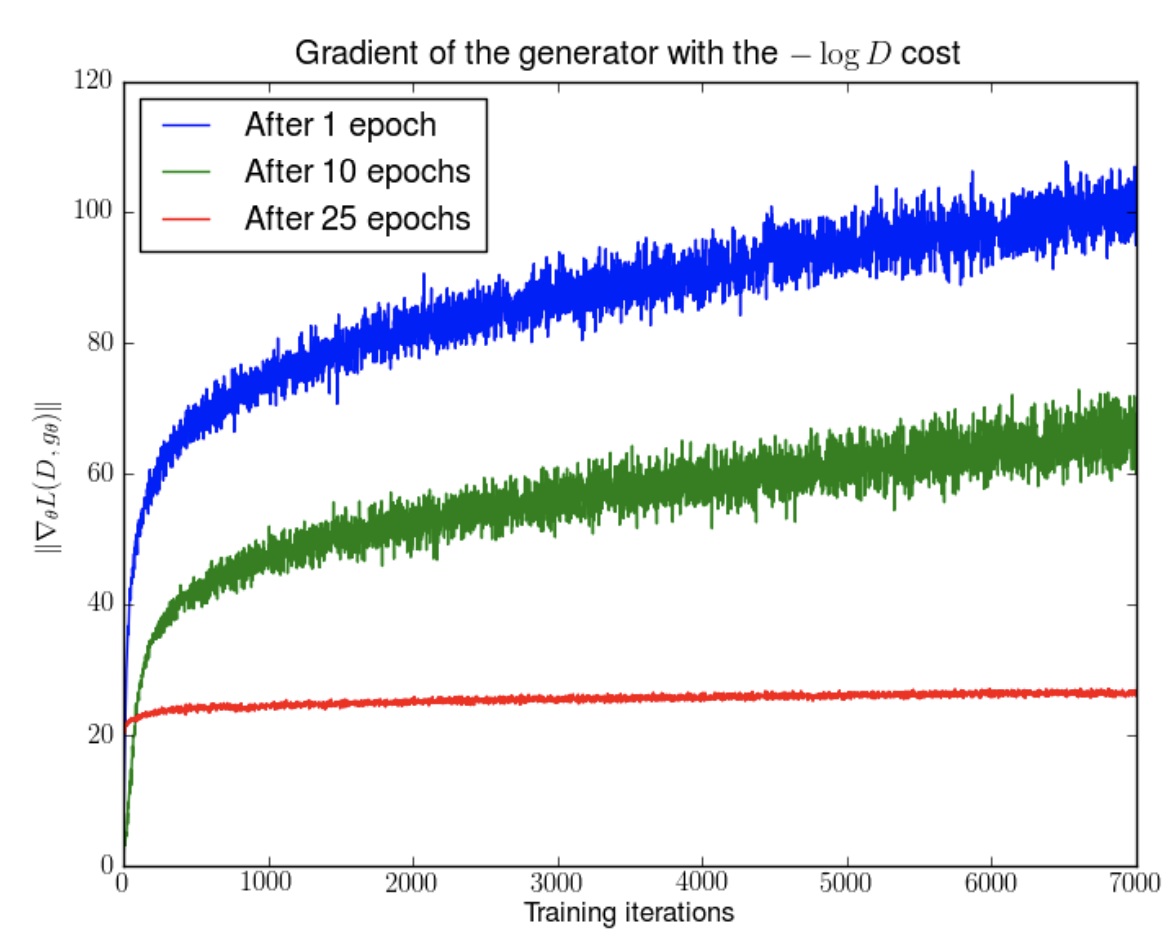
\includegraphics[width=1.0\linewidth]{figs/vanishing_gradients_3}
		\end{figure}
	\end{minipage}
	\vfill
	\hrule\medskip
	{\scriptsize \href{https://arxiv.org/abs/1701.04862}{https://arxiv.org/abs/1701.04862}}
\end{frame}
%=======
\begin{frame}{Likelihood-based vs GAN}
	\begin{block}{GAN objective (for optimal discriminator)}
		\vspace{-0.2cm}
		\[
			V(G, D^*)  = 2JSD(\pi(\bx) || p(\bx | \btheta)) - \log 4.
		\]
	\end{block}
	\begin{block}{Likelihood model objective}
		\vspace{-0.6cm}
		\begin{multline*}
			\max_{\btheta} \log p(\bX | \btheta) \approx \max_{\btheta}\bbE_{\pi(\bx)} \log p(\bx | \btheta) = \\ = \max_{\btheta}\bbE_{\pi(\bx)} \log p(\bx | \btheta) - \bbE_{\pi(\bx)} \log \pi(\bx) = \\ = \max_{\btheta}\bbE_{\pi(\bx)}  \log \frac{p(\bx | \btheta)}{\pi(\bx)}= \min_{\btheta} KL(\pi(\bx) || p(\bx | \btheta))
		\end{multline*}
	\vspace{-0.6cm}
	\end{block}

	What is the difference between $JS$ and $KL$ divergences?
\vfill
\hrule\medskip
{\scriptsize \href{https://arxiv.org/abs/1511.01844}{https://arxiv.org/abs/1511.01844}}
\end{frame}
%=======
\begin{frame}{Mode collapse}
The phenomena where the generator of a GAN collapses to one or few distribution modes.
\begin{figure}
	\centering
	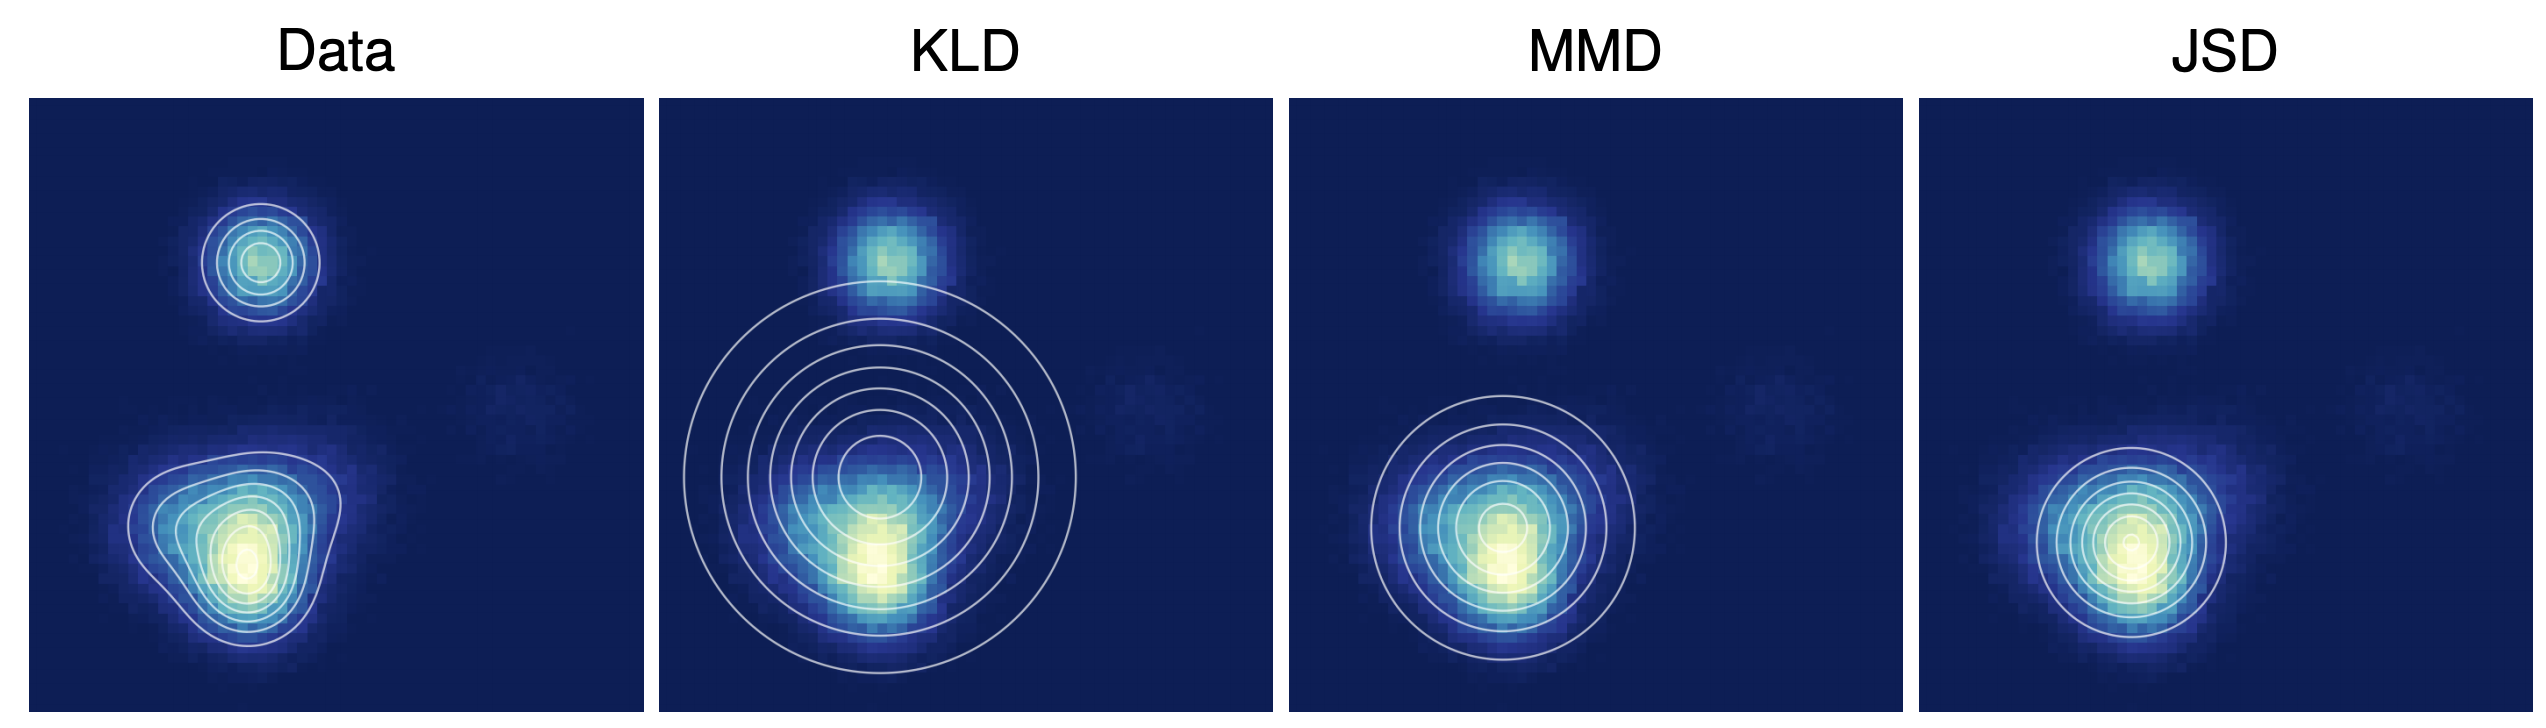
\includegraphics[width=0.9\linewidth]{figs/mode_collapse_1}
\end{figure}
\begin{figure}
	\centering
	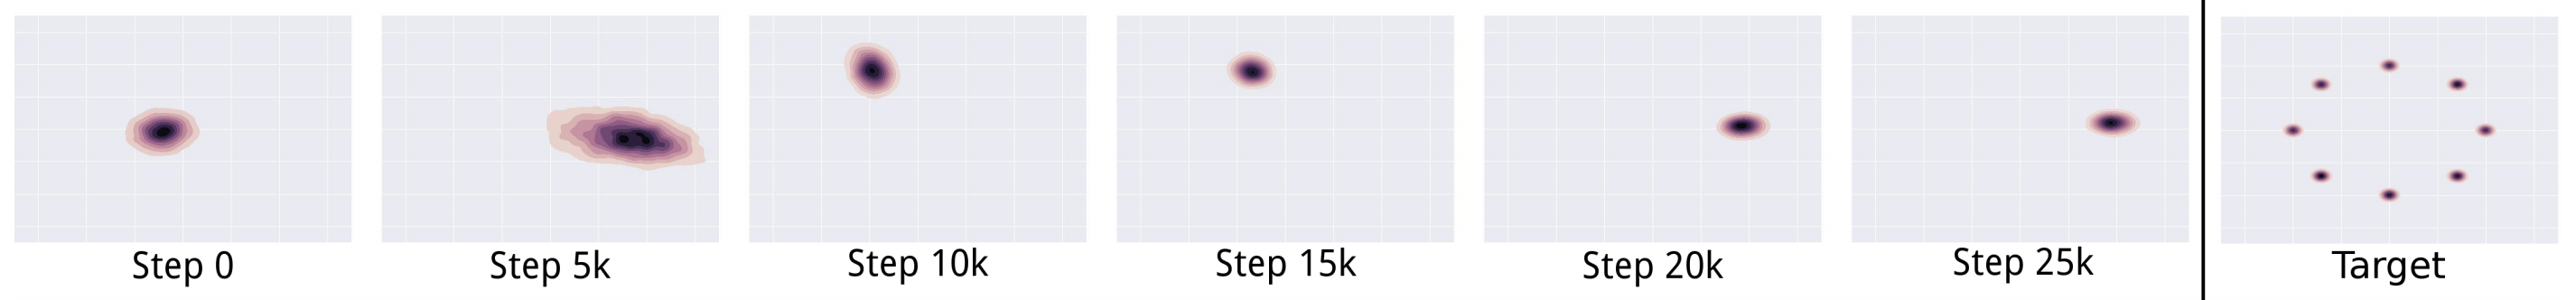
\includegraphics[width=1.0\linewidth]{figs/mode_collapse_3}
\end{figure}
Alternate architectures, adding regularization terms, injecting small noise
perturbations and other millions bags and tricks are used to avoid the mode collapse.
\vfill
\hrule\medskip
{\scriptsize \href{https://arxiv.org/abs/1406.2661}{https://arxiv.org/abs/1406.2661} \\ \href{https://arxiv.org/abs/1611.02163}{https://arxiv.org/abs/1611.02163}}
\end{frame}
%=======
\begin{frame}{Mode collapse}
	\begin{block}{Mode covering vs mode seeking}
		\vspace{-0.2cm}
		\[
			KL(\pi || p) = \int \pi(\bx) \log \frac{\pi(\bx)}{p(\bx)}d\bx, \quad KL(p || \pi) = \int p(\bx) \log \frac{p(\bx)}{\pi(\bx)}d\bx
		\]
		\[
		JSD(\pi || p) = \frac{1}{2} \left[KL \left(\pi(x) || \frac{\pi(\bx) + p(\bx)}{2}\right) + KL \left(p(x) || \frac{\pi(\bx) + p(\bx)}{2}\right) \right]
		\]
		\vspace{-0.4cm}
		\begin{figure}
			\centering
			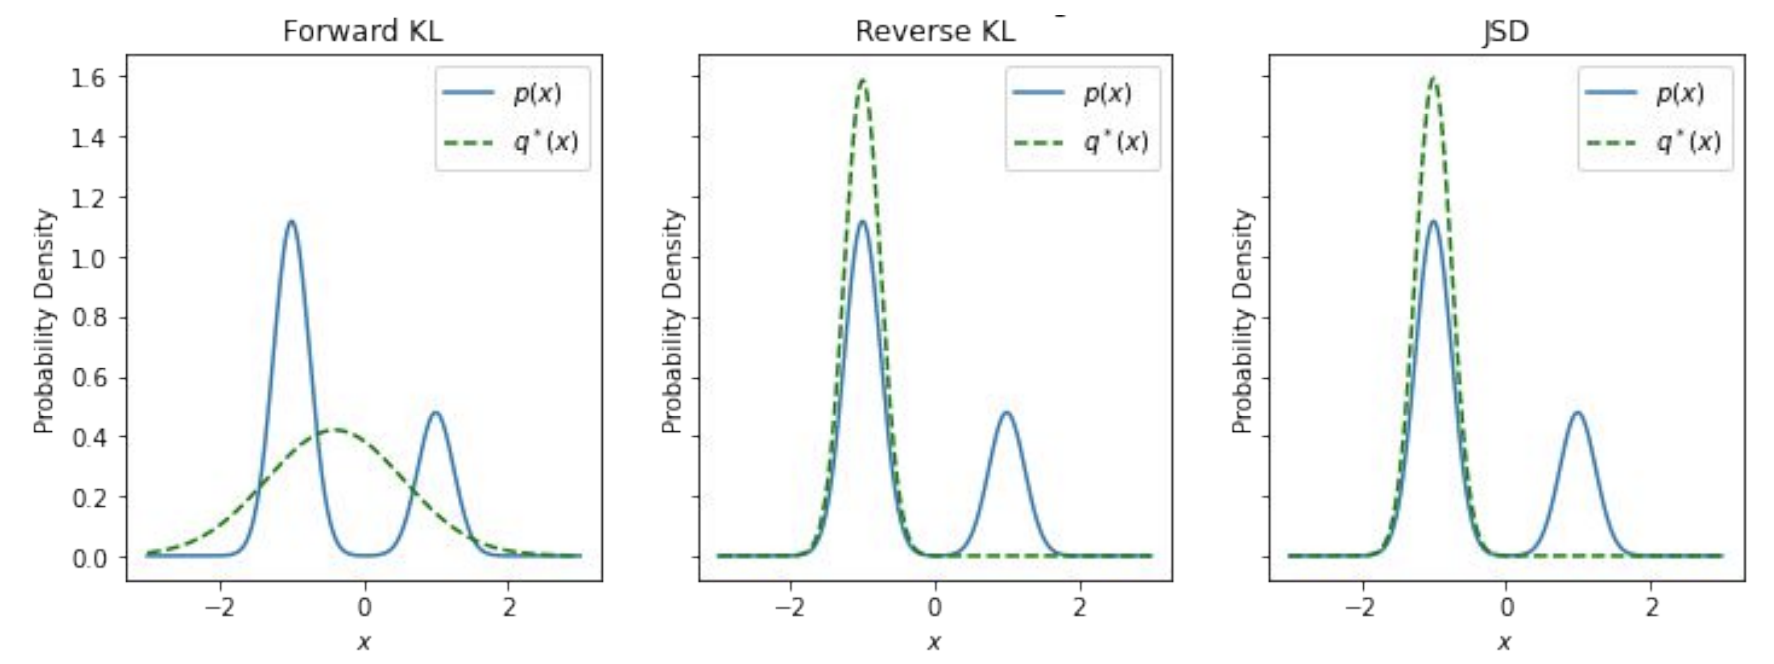
\includegraphics[width=0.7\linewidth]{figs/mode_collapse_2}
		\end{figure}
	\vspace{-0.3cm}
	\end{block}
	\vfill
	\hrule\medskip
	{\scriptsize \href{https://sites.google.com/view/berkeley-cs294-158-sp20/home}{https://sites.google.com/view/berkeley-cs294-158-sp20/home}}
\end{frame}
%=======
\begin{frame}{Vanila GAN results}
	\begin{figure}
		\centering
		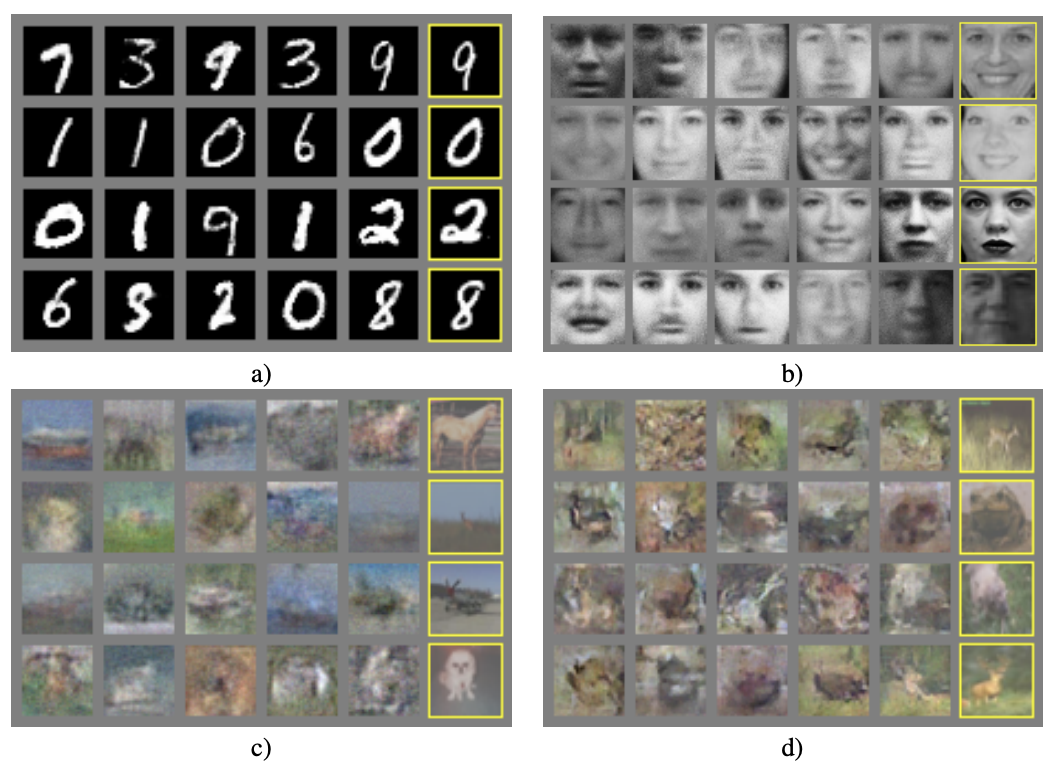
\includegraphics[width=0.95\linewidth]{figs/vanila_gan_results}
	\end{figure}
	\vfill
	\hrule\medskip
	{\scriptsize \href{https://arxiv.org/abs/1406.2661}{https://arxiv.org/abs/1406.2661}}
\end{frame}
%=======
\begin{frame}{Deep Convolutional GAN}
	\begin{figure}
		\centering
		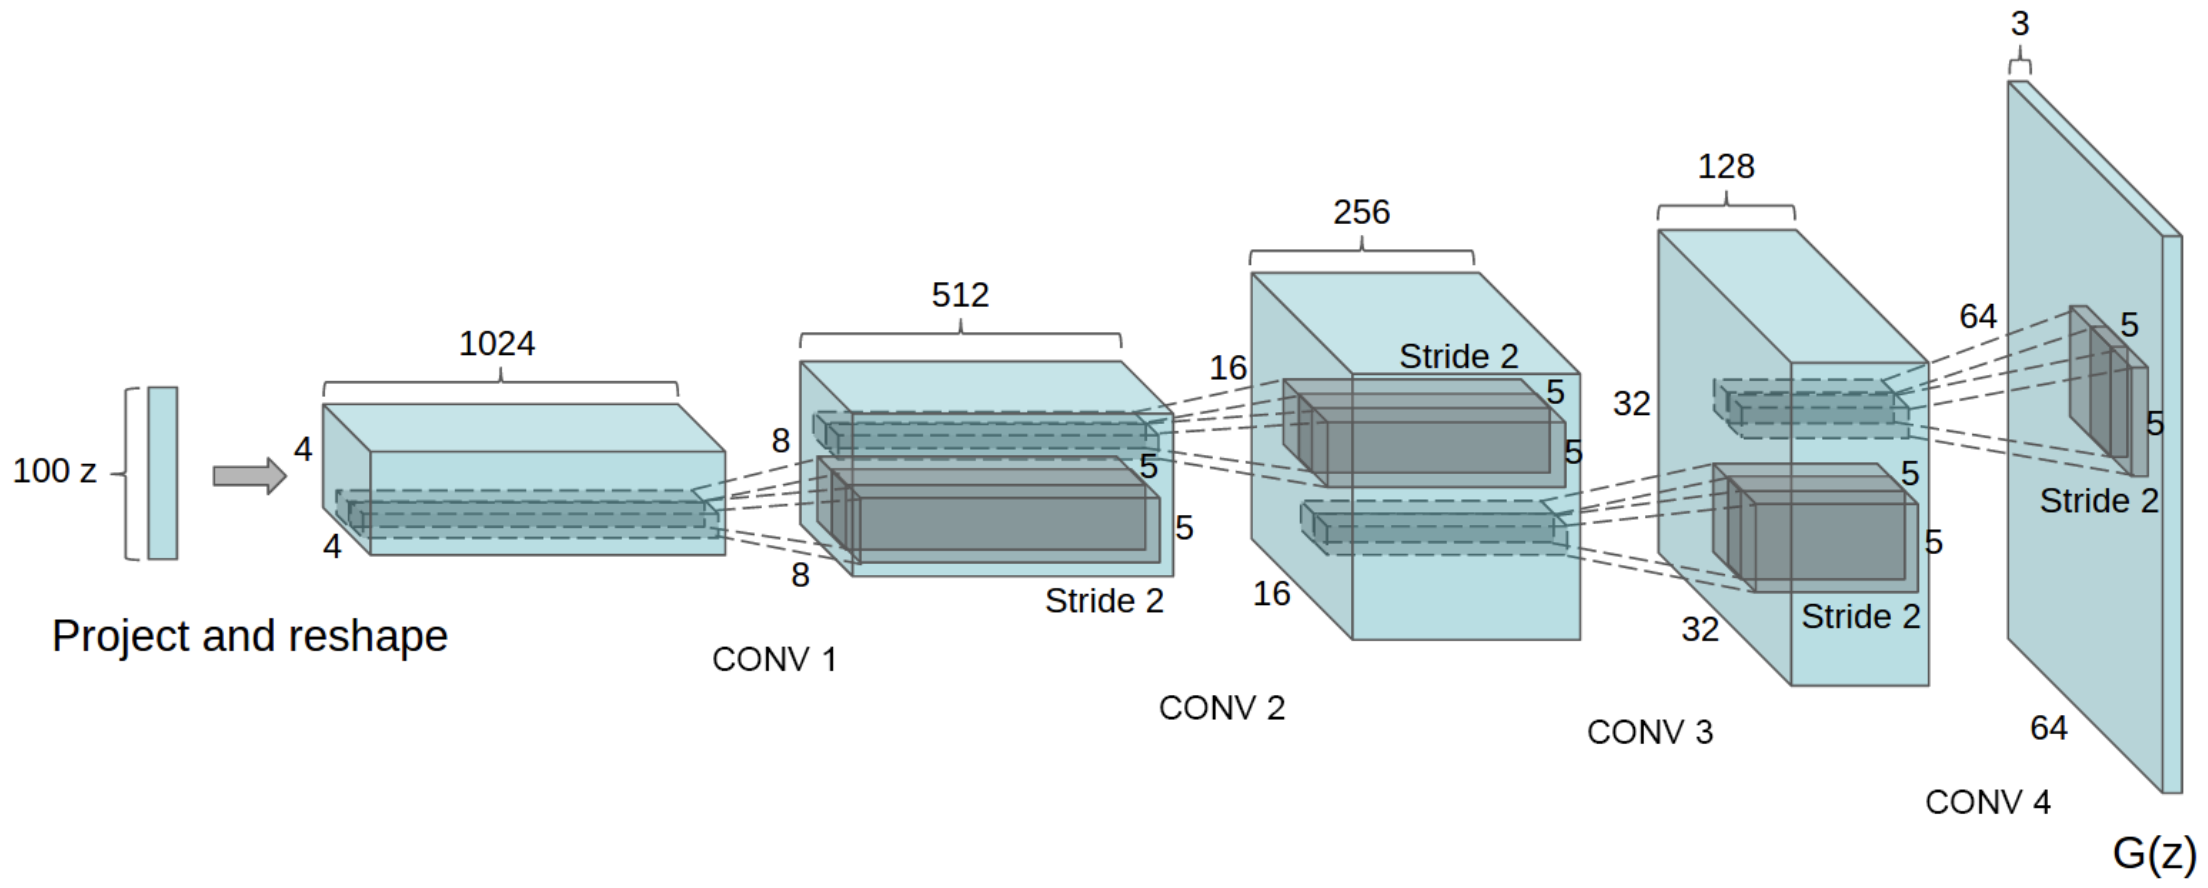
\includegraphics[width=0.8\linewidth]{figs/dcgan_1}
	\end{figure}
	\begin{itemize}
		\footnotesize
		\item  Mean-pooling instead of max-pooling.
		\item Transposed convolutions in the generator for upsampling.
		\item Downsample with strided convolutions and average pooling.
		\item ReLU for generator, Leaky-ReLU (0.2) for discriminator.
		\item Output nonlinearity: tanh for Generator, sigmoid for discriminator.
		\item Batch Normalization used to prevent mode collapse (not applied at the output of $G$ and input of $D$).
		\item Adam: small LR = 2e-4; small momentum: 0.5, batch-size: 128.
	\end{itemize}
	\vfill
	\hrule\medskip
	{\scriptsize \href{https://arxiv.org/abs/1511.06434}{https://arxiv.org/abs/1511.06434}}
\end{frame}
%=======
\begin{frame}{Deep Convolutional GAN}
	\begin{block}{ImageNet samples}
		\begin{figure}
			\centering
			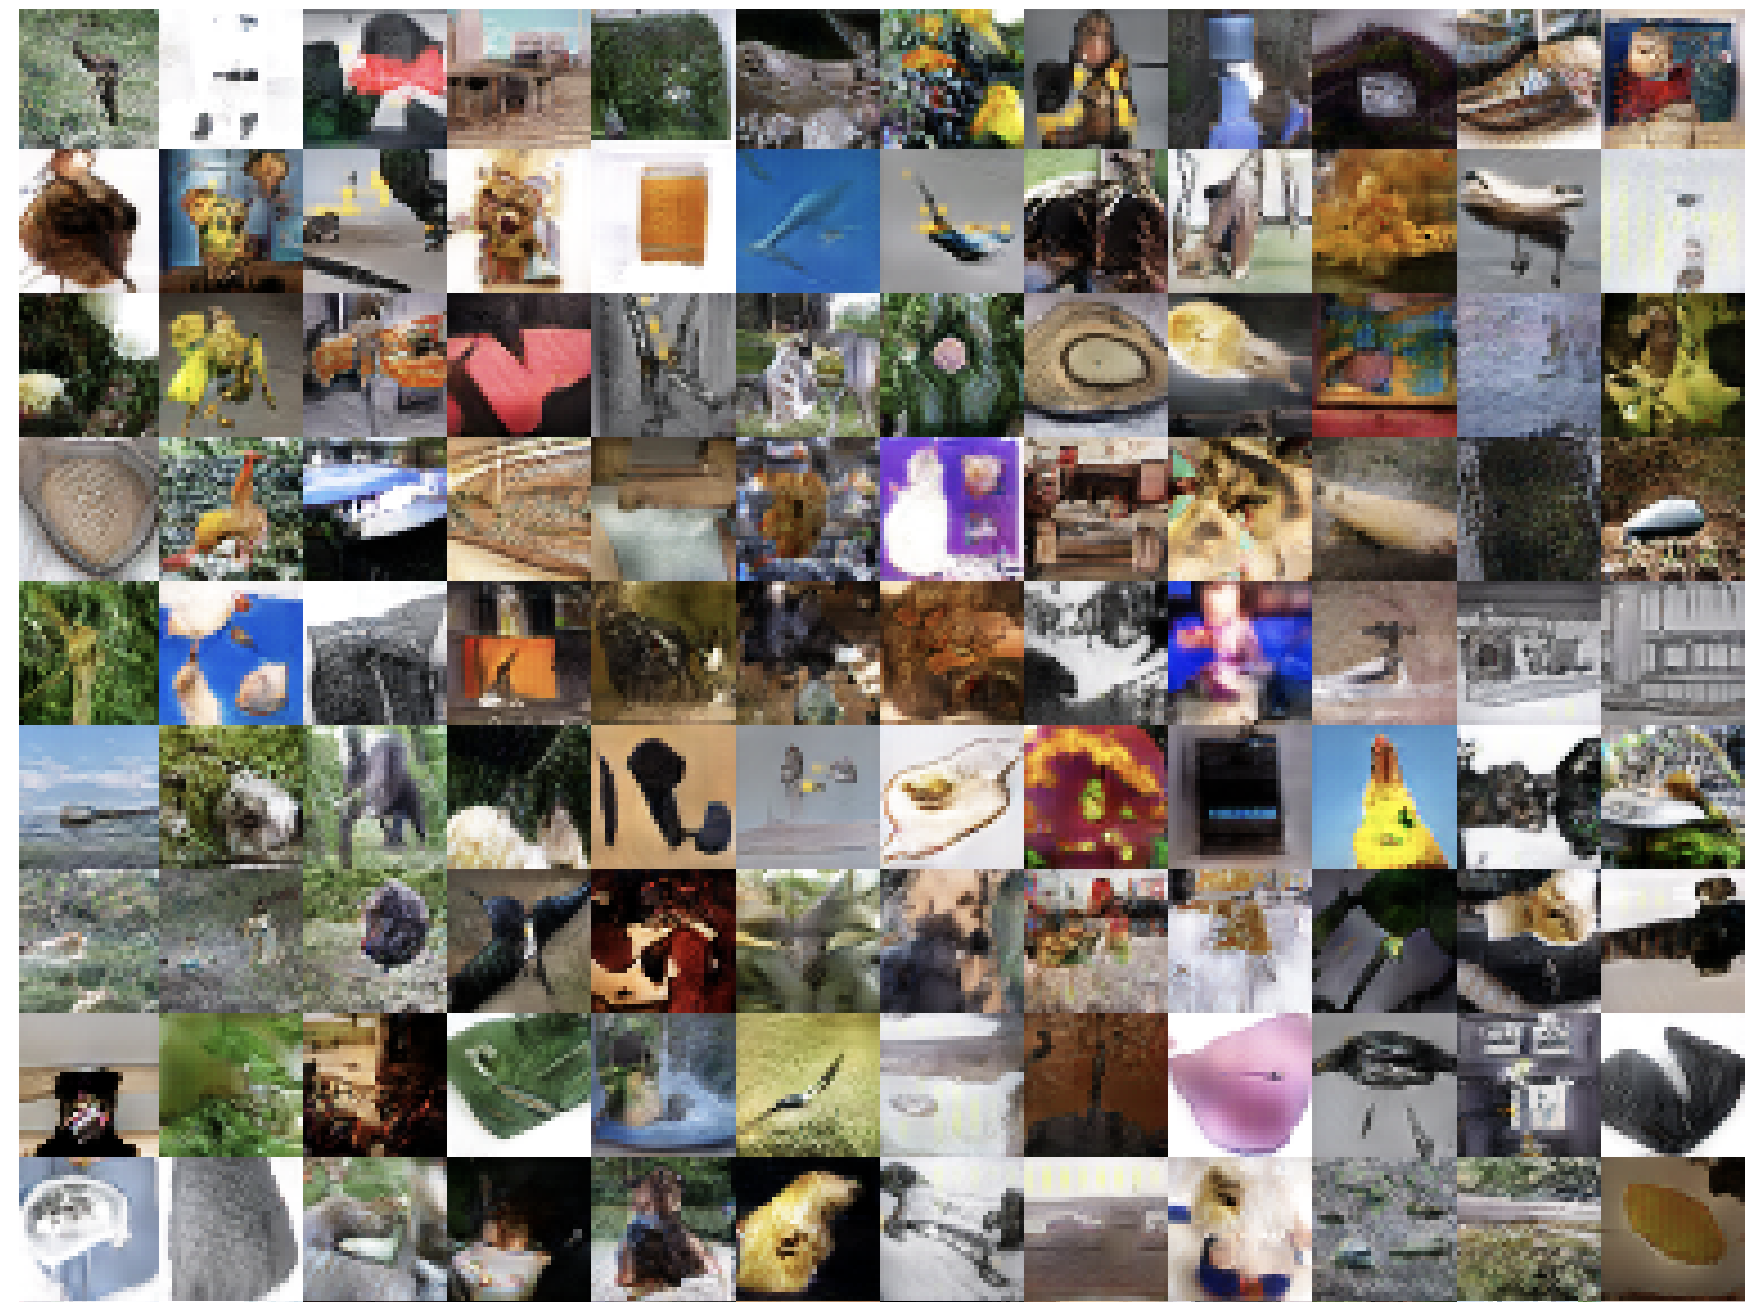
\includegraphics[width=0.8\linewidth]{figs/dcgan_results_1}
		\end{figure}
	\end{block}
	\vfill
	\hrule\medskip
	{\scriptsize \href{https://arxiv.org/abs/1511.06434}{https://arxiv.org/abs/1511.06434}}
\end{frame}
%=======
\begin{frame}{Deep Convolutional GAN}
	\begin{block}{Smooth interpolations}
		\begin{figure}
			\centering
			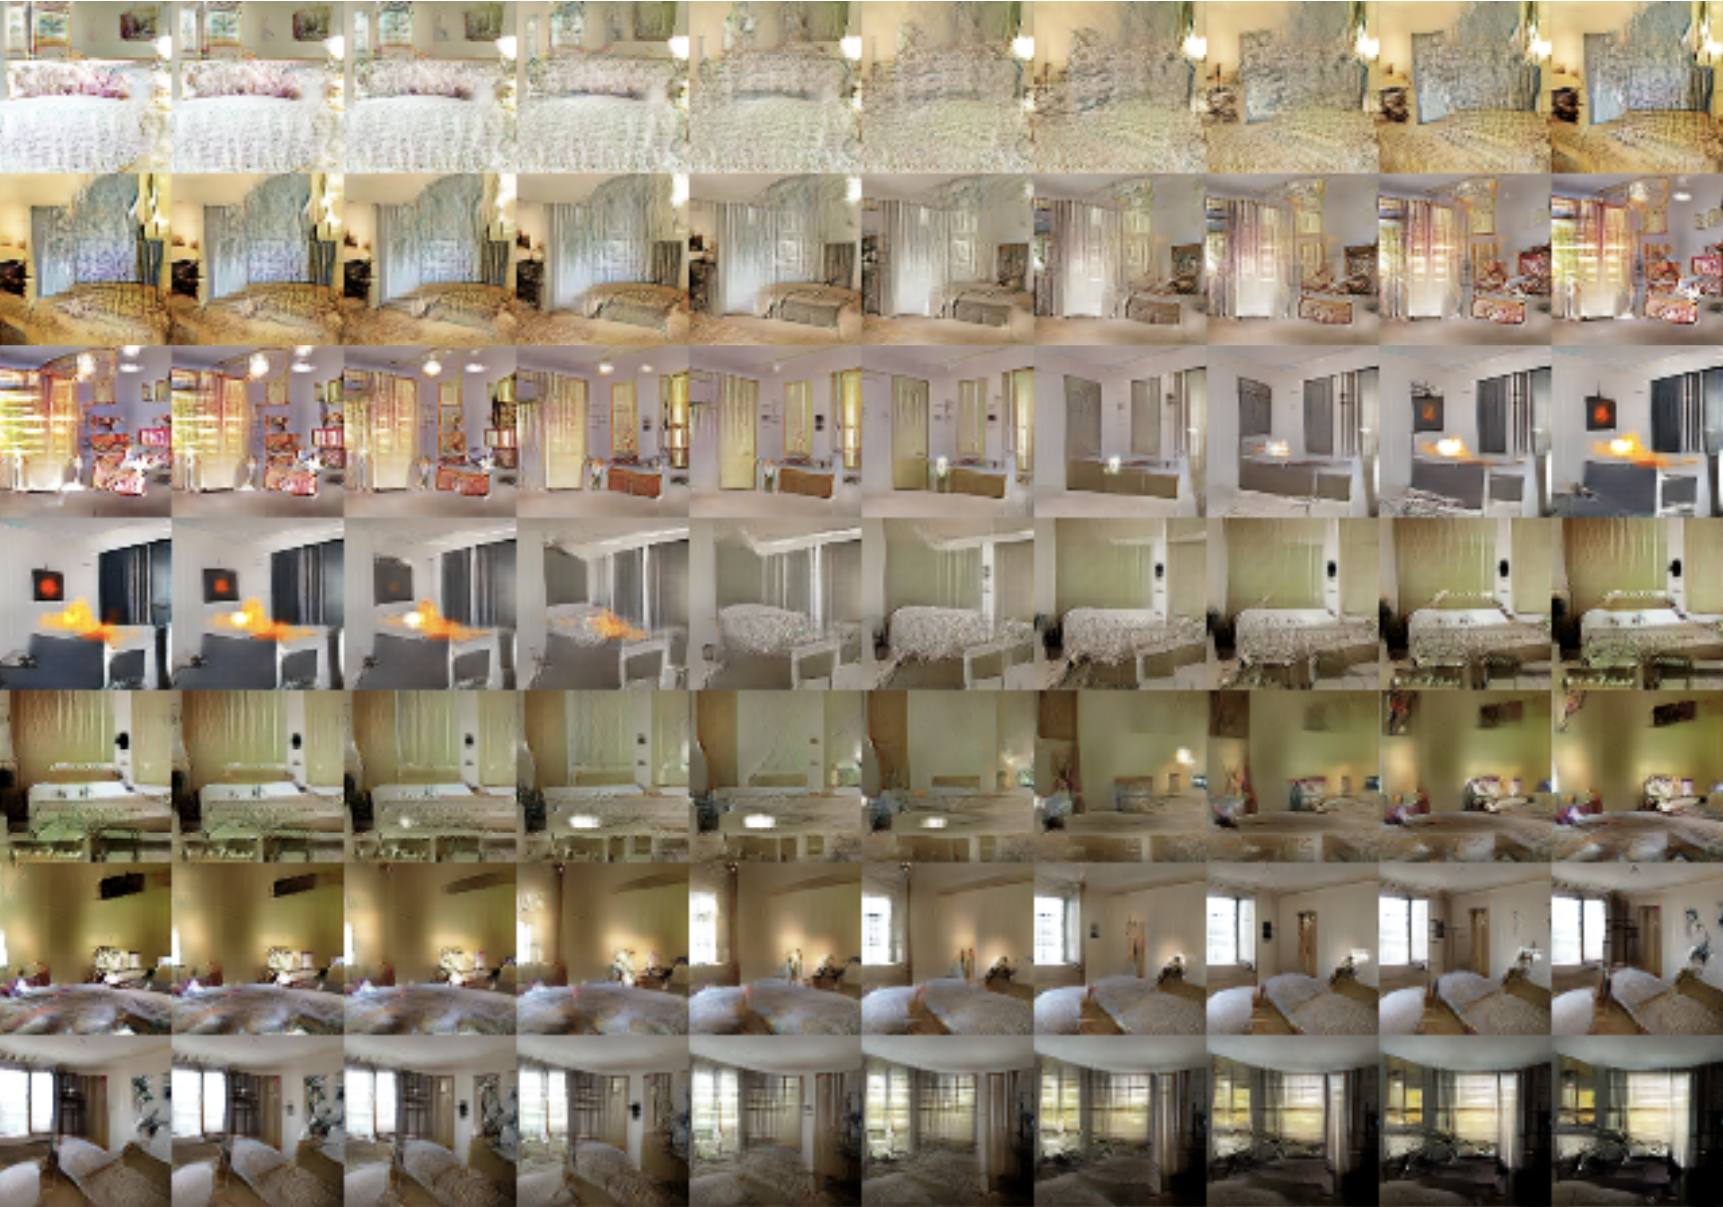
\includegraphics[width=0.8\linewidth]{figs/dcgan_results_2}
		\end{figure}
	\end{block}
	\vfill
	\hrule\medskip
	{\scriptsize \href{https://arxiv.org/abs/1511.06434}{https://arxiv.org/abs/1511.06434}}
\end{frame}
%=======
\begin{frame}{Deep Convolutional GAN}
	\begin{block}{Vector arithmetic}
		\begin{figure}
			\centering
			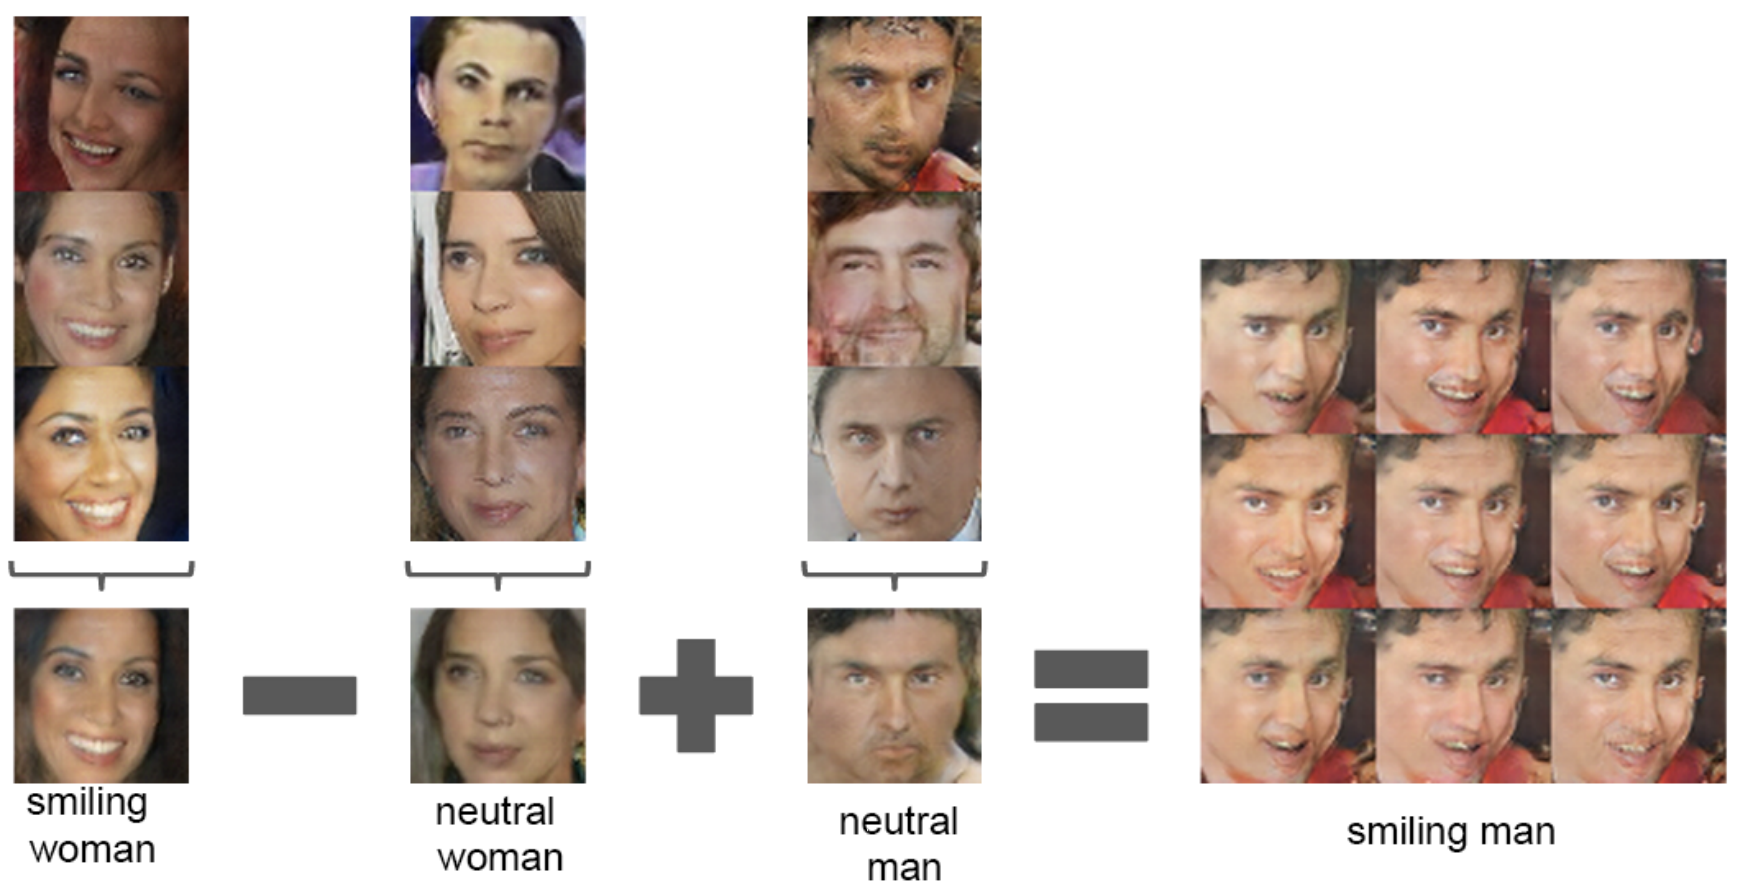
\includegraphics[width=1.0\linewidth]{figs/dcgan_results_3}
		\end{figure}
	\end{block}
	\vfill
	\hrule\medskip
	{\scriptsize \href{https://arxiv.org/abs/1511.06434}{https://arxiv.org/abs/1511.06434}}
\end{frame}
%=======
\begin{frame}{Deep Convolutional GAN}
	\begin{block}{Mode collapse}
		\begin{figure}
			\centering
			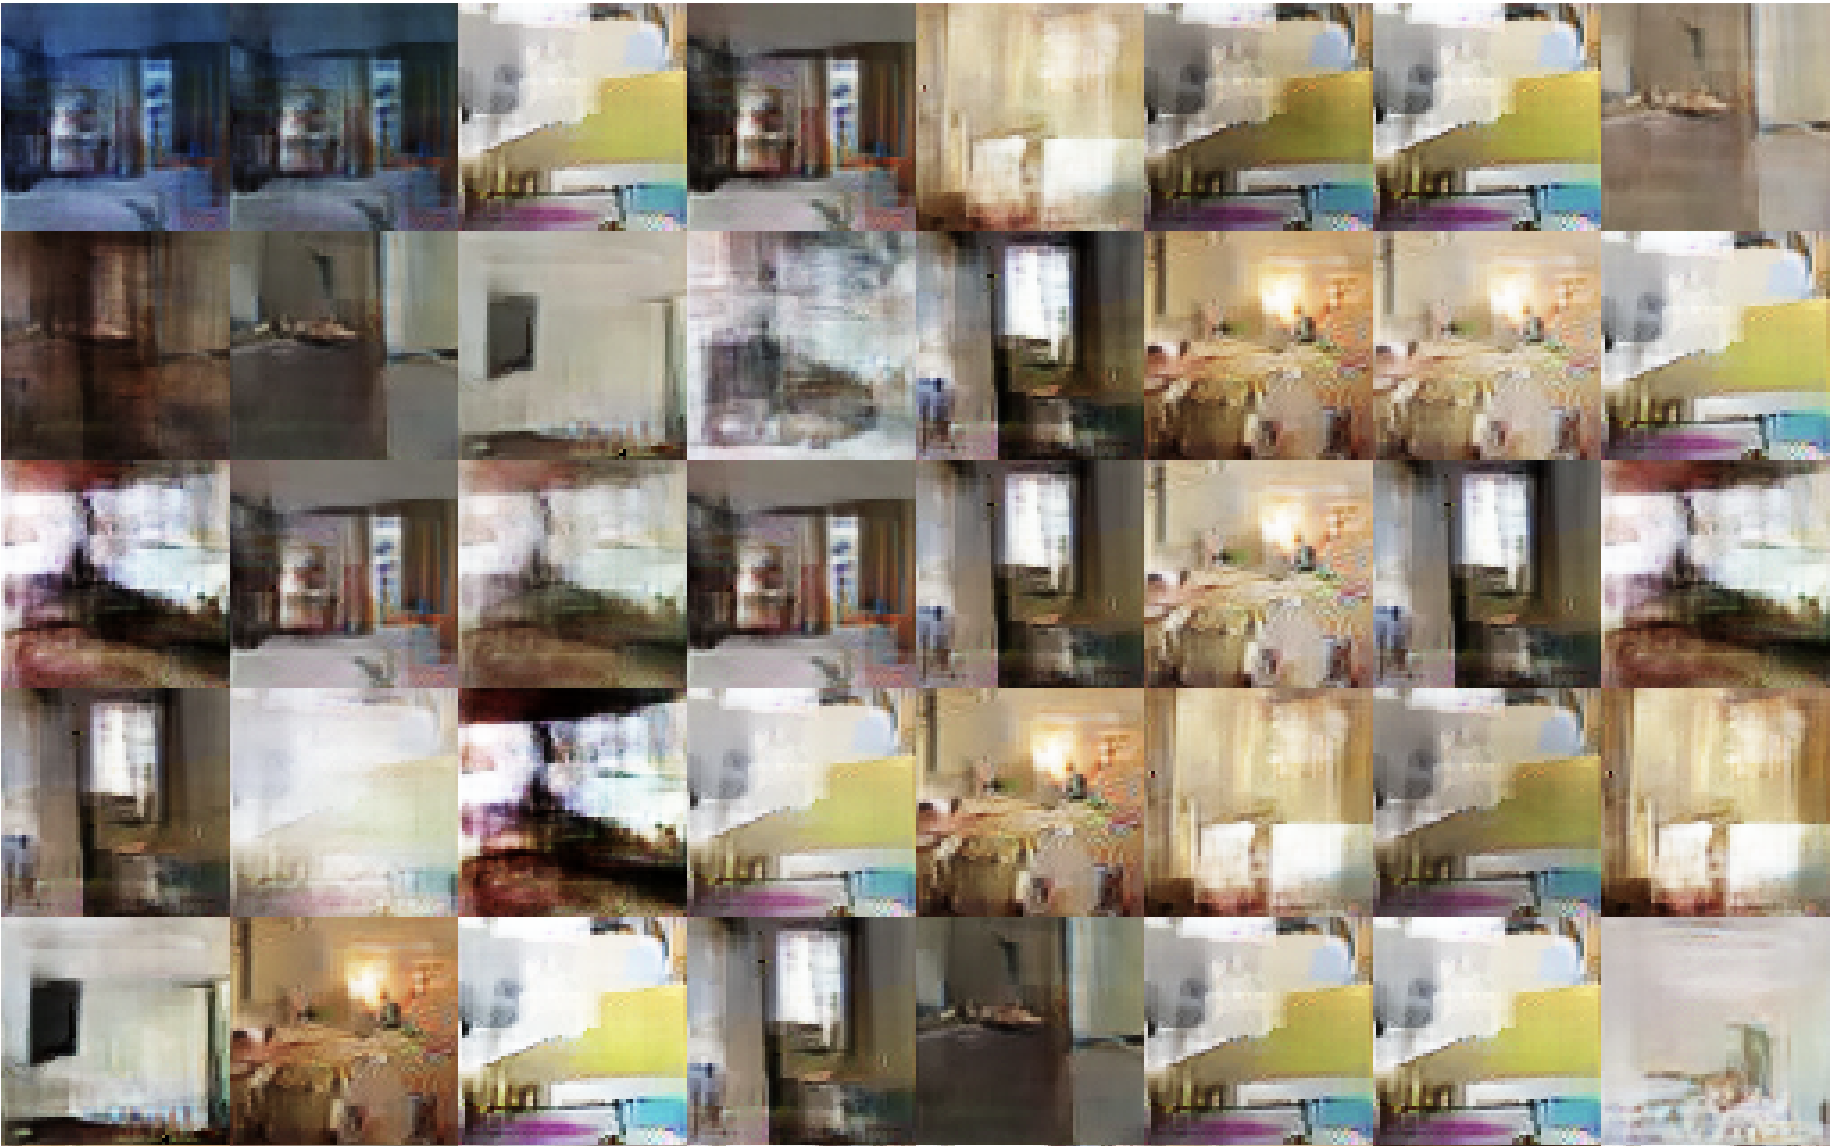
\includegraphics[width=0.95\linewidth]{figs/mode_collapse_4}
		\end{figure}
	\end{block}
	\vfill
	\hrule\medskip
	{\scriptsize \href{https://arxiv.org/abs/1701.07875}{https://arxiv.org/abs/1701.07875}}
\end{frame}
%=======
\begin{frame}{Improved techniques for training GANs}
	\begin{itemize}
		\item Feature matching
		\[
			\cL_G = \| \bbE_{\pi(\bx)} \mathbf{d}(\bx) - \bbE_{p(\bz)} \mathbf{d}(G(\bz)) \|_2^2
		\]
		Here $\mathbf{d}(\bx)$ -- intermediate layer of discriminator. Matching the learned discriminator statistics instead of the output of the discriminator. Helps to avoid the vanishing gradients for sufficiently good discriminator.
		\item Historical averaging adds extra loss term for generator and discriminator losses
		\vspace{-0.2cm}
		\[
		 \| \btheta - \frac{1}{T}\sum_{t=1}^T \btheta_t\|^2_2.
		\]
		Here $\btheta_t$ -- value of parameters at the previous step $t$. It allows to stabilize training procedure.
	\end{itemize}
	\vfill
	\hrule\medskip
	{\scriptsize \href{https://arxiv.org/abs/1606.03498}{https://arxiv.org/abs/1606.03498}}
\end{frame}
%=======
\begin{frame}{Improved techniques for training GANs}
	\begin{itemize}
		\item One-sided label smoothing. Instead of using one-hot labels in classification, use $(1 - \alpha)$ for real data (the generated samples are not smoothed).
		\[
			D^*(\bx) = \frac{(1 - \alpha )\pi(\bx)}{\pi(\bx) + p(\bx | \btheta)}
		\]
		\item Virtual batch normalization. BatchNorm makes samples within minibatch are highly correlated.
		\begin{figure}
			\centering
			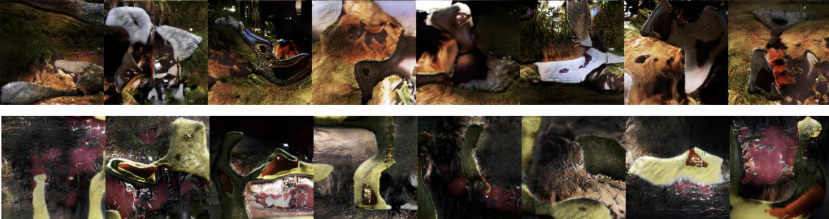
\includegraphics[width=0.6\linewidth]{figs/virtual_batch_norm}
		\end{figure}
	Use reference fixed batch to compute the normalization statistics. To avoid overfitting construct batch with the reference batch and the current sample. 
	\end{itemize}
	\vfill
	\hrule\medskip
	{\scriptsize \href{https://arxiv.org/abs/1606.03498}{https://arxiv.org/abs/1606.03498}}
\end{frame}
%=======
\begin{frame}{Informal theoretical results}
	\begin{itemize}
		\footnotesize
		\item Since $\bz$ usually has lower dimensionality compared to $\bx$, manifold $G(\bz)$ has a measure 0 in $\bx$ space. Hence, support of $p(\bx | \btheta)$ lies on low-dimensional manifold.
		\item Distribution of real images $\pi(\bx)$ is also concentrated on a low dimensional manifold.
		\begin{figure}
			\centering
			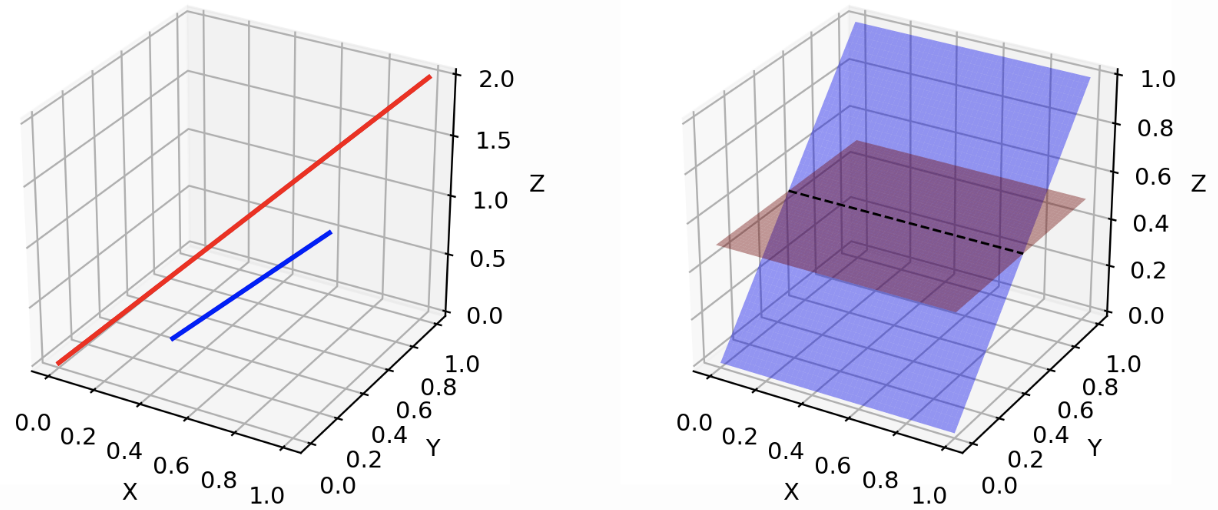
\includegraphics[width=0.5\linewidth]{figs/low_dim_manifold}
		\end{figure}
		\item If $\pi(\bx)$ and $p(\bx | \btheta)$ have disjoint supports, then there is a smooth optimal discrimator. In this case we won’t really be able to learn anything by backproping through it.
		\item For such low-dimensional disjoint manifolds
		\[
			KL(\pi || p) = KL(p || \pi) = \infty, \quad JSD(\pi || p) = \log 2
		\]
		\item Adding continuous noise to the inputs of the discriminator smoothes the distributions of the probability mass.
	\end{itemize}
	\vfill
	\hrule\medskip {\scriptsize \href{https://lilianweng.github.io/lil-log/2017/08/20/from-GAN-to-WGAN.html}{https://lilianweng.github.io/lil-log/2017/08/20/from-GAN-to-WGAN.html} \\ 
	\href{https://arxiv.org/abs/1701.04862}{https://arxiv.org/abs/1701.04862}}
\end{frame}
%=======
\begin{frame}{Wasserstein distance (discrete)}
	Also called Earth Mover's distance.
	The minimum cost of moving and transforming a pile of dirt in the shape of one probability distribution to the shape of the other distribution.
	\begin{figure}
		\centering
		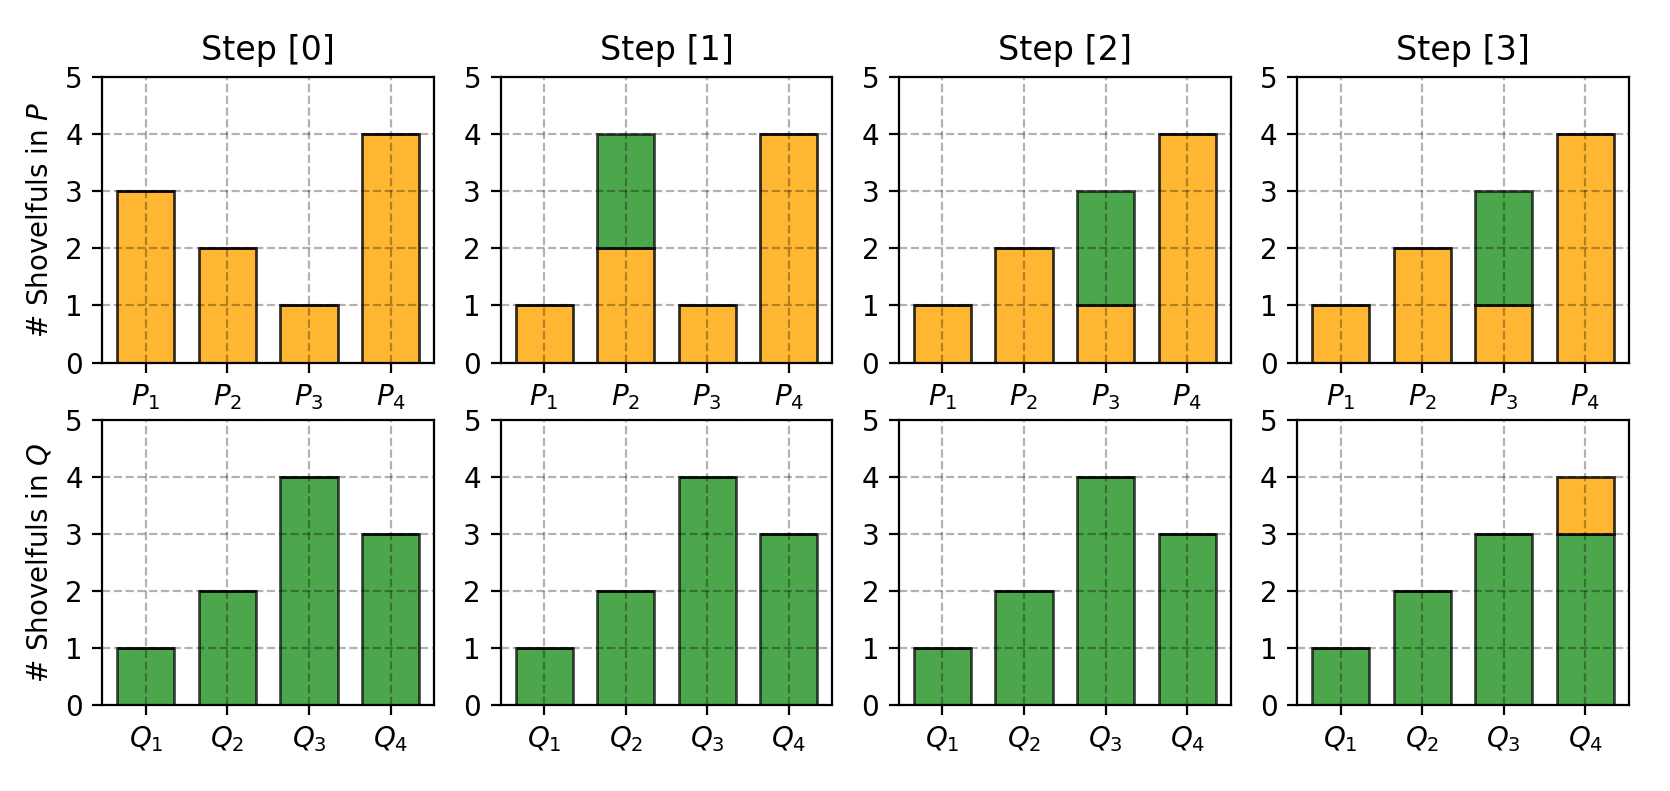
\includegraphics[width=.9\linewidth]{figs/EM_distance_discrete}
	\end{figure}
	\[
		W(P, Q) = 2 \text{(step 1)} + 2 \text{(step 2)} + 1 \text{(step 3)}  = 5
	\]
	\vfill
	\hrule\medskip 
	{\scriptsize \href{https://lilianweng.github.io/lil-log/2017/08/20/from-GAN-to-WGAN.html}{https://lilianweng.github.io/lil-log/2017/08/20/from-GAN-to-WGAN.html}}
	
\end{frame}
%=======
\begin{frame}{Wasserstein distance}
	\[
		W(\pi, p) = \inf_{\gamma \in \prod(\pi, p)} \bbE_{(\bx, \by) \sim \gamma} \| \bx - \by \| =  \inf_{\gamma \in \prod(\pi, p)} \int \| \bx - \by \| \gamma (\bx, \by) d \bx d \by
	\]
	\begin{itemize}
		\item $\prod(\pi, p)$ -- the set of all joint distributions $\gamma (\bx, \by)$ with marginals $\pi$ and $p$ ($\int \gamma(\bx, \by) d \bx = p(\by)$, $\int \gamma(\bx, \by) d \by = \pi(\bx)$)
		\item $\gamma(\bx, \by)$ -- transportation plan (the amount of "dirt" that should be transported from point $\bx$ to point $\by$).
		\item $\gamma(\bx, \by)$ -- the amount, $\|\bx - \by \|$-- the distance.
	\end{itemize}
	For better understanding of transportation plan function $\gamma$, try to write down the plan for previous discrete case.
	\vfill
	\hrule\medskip 
	{\scriptsize \href{https://arxiv.org/abs/1701.07875}{https://arxiv.org/abs/1701.07875}}
\end{frame}
%=======
\begin{frame}{Wasserstein distance vs KL vs JSD}
	
	\begin{minipage}[t]{0.48\columnwidth}
		\vspace{0.1cm}
		Consider 2d distributions
		\[
			\pi(x, y) = (0, U[0,1])
		\]	
		\[
			p(x, y | \theta) = (\theta, U[0, 1])
		\]
	\end{minipage}%
	\begin{minipage}[t]{0.52\columnwidth}
		\begin{figure}
			\centering
			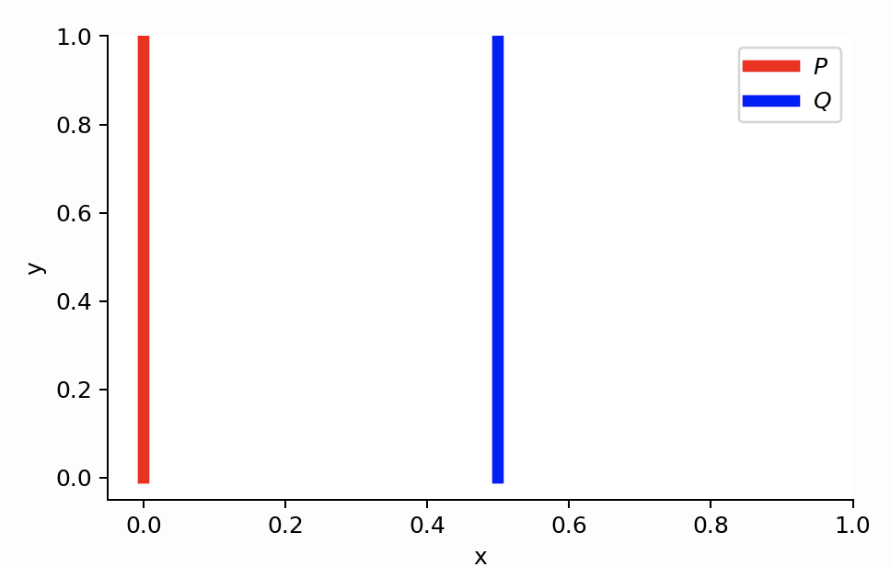
\includegraphics[width=0.8\linewidth]{figs/w_kl_jsd}
		\end{figure}
	\end{minipage}
	\begin{itemize}
		\footnotesize
		\item $\theta = 0$.
		Distributions are the same 
		\[
			KL(\pi || p) = KL(p || \pi) = JSD(p || \pi) = W(\pi, p) = 0
		\]
		\item $\theta \neq 0$
		\[
			KL(\pi || p) = \int_{U[0, 1]} 1 \log \frac{1}{0} d y = \infty = KL(p || \pi)
		\]
		\[
			JSD(\pi || p) = \frac{1}{2}\left( \int_{U[0, 1]}1 \log \frac{1}{1/2} dy + \int_{U[0, 1]}1 \log \frac{1}{1/2} dy \right) = \log 2
		\]
		\[
			W(\pi, p) = |\theta|
		\]
	\end{itemize}
	\vfill
	\hrule\medskip 
	{\scriptsize  \href{https://lilianweng.github.io/lil-log/2017/08/20/from-GAN-to-WGAN.html}{https://lilianweng.github.io/lil-log/2017/08/20/from-GAN-to-WGAN.html} \\ \href{https://arxiv.org/abs/1701.07875}{https://arxiv.org/abs/1701.07875}}
\end{frame}
%=======
\begin{frame}{Wasserstein distance vs KL vs JSD}
	\begin{block}{Theorem 1}
		Let $G(\bz, \btheta)$ be any feedforward neural network, and $p(\bz)$ a prior over $\bz$ such that $\bbE_{\bz \sim p(\bz)}
		\|\bz\| < \infty$. Then therefore $W(\pi, p)$ is continuous everywhere and differentiable almost everywhere.
	\end{block}
	\begin{block}{Theorem 2}
		Let $\pi$ be a distribution on a compact space $\cX$ and $\{p_t\}_{t=1}^\infty$ be a sequence of distributions on $\cX$. 
		\begin{align}
			KL(\pi || p_t) &\rightarrow 0 \, (\text{or }KL (p_t || \pi) \rightarrow 0) \\
			JSD(\pi || p_t) &\rightarrow 0 \\
			W(\pi || p_t) &\rightarrow 0
		\end{align}
		
		Then, considering limits as $t \rightarrow \infty$, (1) implies (2), (2) implies (3).
	\end{block}
	\vfill
	\hrule\medskip 
	{\scriptsize \href{https://arxiv.org/abs/1701.07875}{https://arxiv.org/abs/1701.07875}}
\end{frame}
%=======
\begin{frame}{References}
{\tiny
\begin{itemize}
	\item A note on the evaluation of generative models \\
	\href{https://arxiv.org/abs/1511.01844}{https://arxiv.org/abs/1511.01844} \\
	\textbf{Summary:} Reviews properties relating to the evaluation and interpretation of generative models. Different divergences \\ leads to different properties. Log-likelihood values are not always meaningful in terms of samples quality.
	
	\item Generative Adversarial Nets \\
	\href{https://arxiv.org/abs/1406.2661}{https://arxiv.org/abs/1406.2661} \\
	\textbf{Summary:} GAN framework is proposed. Theorem about oprimal discriminator has been proved. Some theroretical analysis \\ has been made. Experiments were carried out only on small datasets.
	
	\item \textbf{DCGAN}: Unsupervised Representation Learning with Deep Convolutional Generative Adversarial Networks \\
	\href{https://arxiv.org/abs/1511.06434}{https://arxiv.org/abs/1511.06434} \\
	\textbf{Summary:} First successful application of GAN for CNN models. Suggest simple architectural guides to train such models. 
	
	\item Improved techniques for training GANs \\
	\href{https://arxiv.org/abs/1606.03498}{https://arxiv.org/abs/1606.03498} \\
	\textbf{Summary:} Proposed techniques to improve gan training. Feature matching, minibatch discrimination, historical averaging, one-sided label smoothing, virtual batchnorm.
	
	\item Towards principled methods for training generative adversarial networks \\
	\href{https://arxiv.org/abs/1701.04862}{https://arxiv.org/abs/1701.04862} \\
	\textbf{Summary:} Low-dimensional manifolds are likely be disjoint. In this case KL and JSD are bad objectives. Analyzes \\ theoretically the vanishing gradient problems. Propose adding noise to samples.
	
	\item \textbf{WGAN}: Wasserstein GAN \\
	\href{https://arxiv.org/abs/1701.07875}{https://arxiv.org/abs/1701.07875} \\
	\textbf{Summary:} Proposed Earth-Mover distance as divergence measure. It shows theoretically that EM distance could be better \\ than KL, JS and TV measures. Kantorovich-Rubinstein duality gives the new objective. All we need to enforce is Lipschitz \\ continuity (e.x. by gradient clipping).
\end{itemize}
}
\end{frame}
%=======
\end{document} 